\section{Particle filters for linear/Gaussian systems}
\subsection{Task 2a}
\subsubsection{Part 1}

\texttt{pfFilter} function offers $ xfp $, which is the posterior means of particle filter , and $ Pfp $, which is posterior error covariances of particle filter.

To calculate MSE, there is a function name as \texttt{mse} which is offered by Matlab.

The key codes are here:

\begin{lstlisting}
    % figure;hold on;
    [xfpre, Pfpre, Xpre, Wpre] = pfFilter(x_0, P_0, Y, f, Q, h, R, ParticleNum, 1, myplot);
    % title('Resample')
    % figure;hold on;
    [xfp, Pfp, Xp, Wp] = pfFilter(x_0, P_0, Y, f, Q, h, R, ParticleNum, 0, myplot);
    % title('Noresample')
    
    %xfp is mean and Pfp is covariance
    disp('KF mse:')
    mse(X(2:end)-xf)
    disp('PF with resample')
    mse(X(2:end)-xfpre)
    disp('PF without resample')
    mse(X(2:end)-xfp)
\end{lstlisting}

I have tried a couple of numbers to see the trend of these MSEs:

\begin{table}[htbp]
	\centering
	\caption{MSE and Number of Particles }
    \label{MSE}
	\begin{tabular}{cccc}
		\hline
         & KF& PF  & PF-resample \\ \hline
		 Np=20& 1.3898 & 2.4238 & 3.6028 \\
		 Np=30& 1.4601 & 1.7728 & 5.6019 \\
         Np=40& 2.0392 & 2.2256 & 7.1138 \\
		 Np=50& 1.7932 & 1.7836 & 4.8646 \\ \hline
	\end{tabular}
\end{table}

From table \ref{MSE}, the PF with resample can reach the precision of KF around the number of particles equal to 50.


\begin{figure}[H]
 \centering
 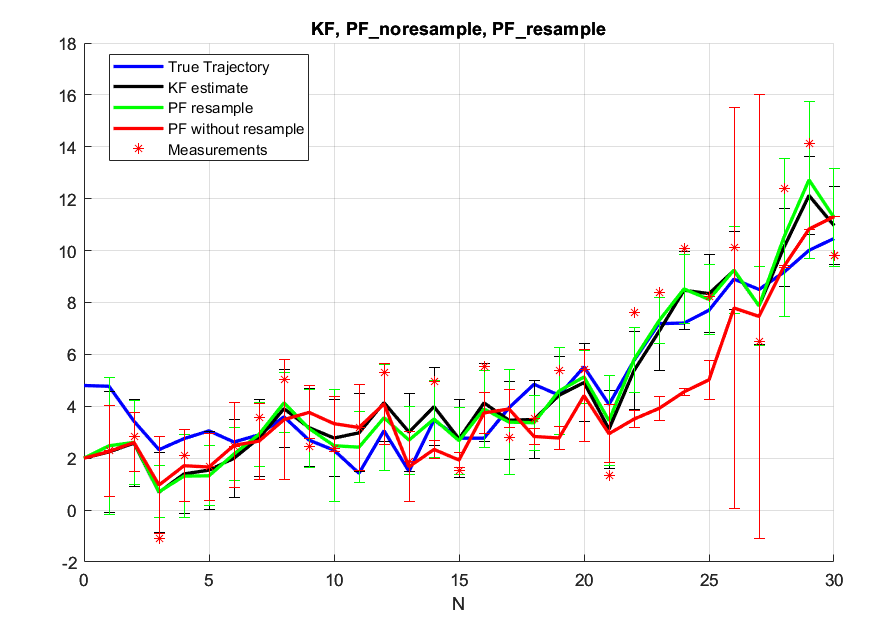
\includegraphics[width=0.7\textwidth]{images/2a.png}
 \caption{Filters and True trajectory}
 \label{2a}
\end{figure}

\subsubsection{Part 2}
I chose three values: $ k=1, 14, 28 $

After some tuning, set $ \sigma = 2.5 $, and the pictures are:

\begin{figure}[H]
    \centering
    \begin{minipage}[b]{0.4\textwidth}
      \centering
      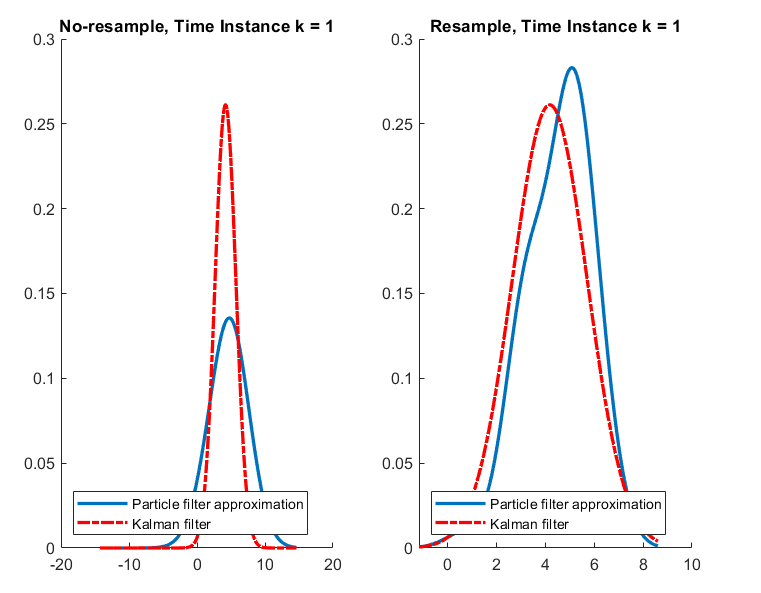
\includegraphics[width=\textwidth]{images/k=1.png}
      \caption{K=1}
      \label{fig:K=1}
    \end{minipage}
    \hfill
    \begin{minipage}[b]{0.4\textwidth}
      \centering
      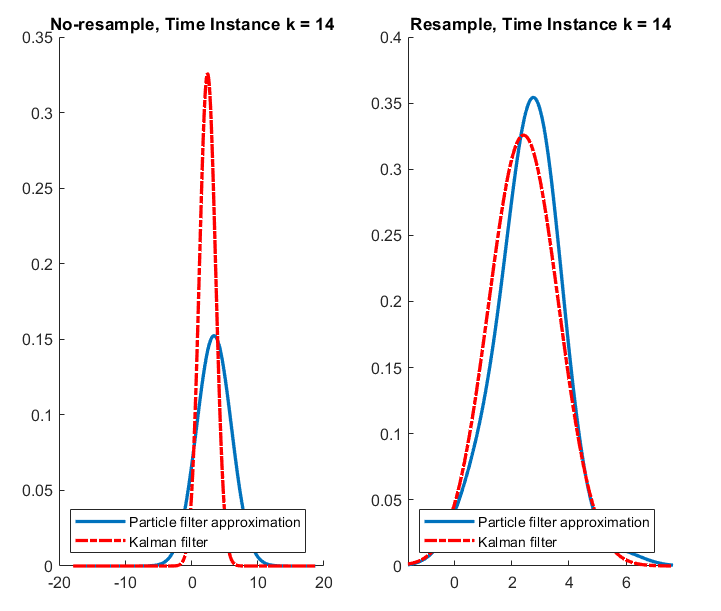
\includegraphics[width=\textwidth]{images/K=14.png}
      \caption{K=14}
      \label{fig:K=14}
    \end{minipage}
    \hfill
    \begin{minipage}[b]{0.4\textwidth}
      \centering
      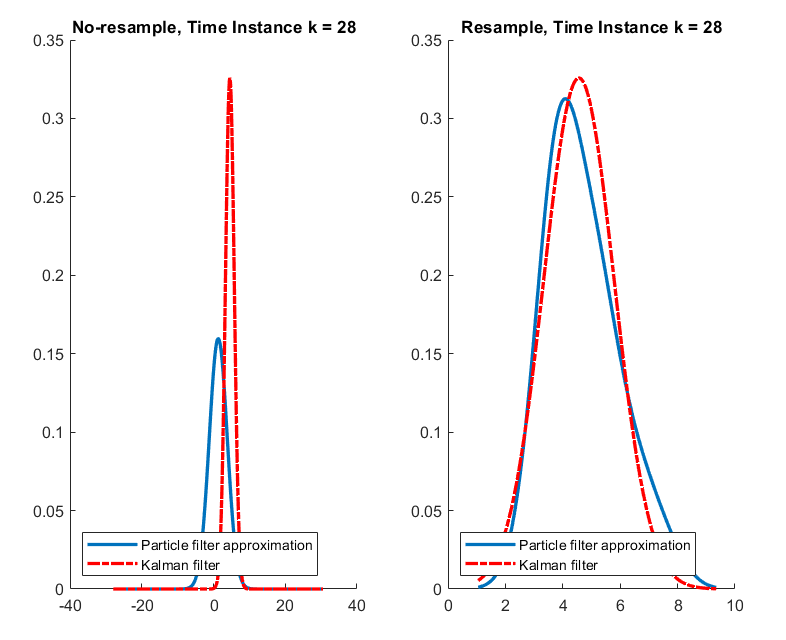
\includegraphics[width=\textwidth]{images/K=28.png}
      \caption{K=28}
      \label{fig:K=28}
    \end{minipage}
   \end{figure}
   
With the step going from 1 to 28, the resampled filter goes closer to the KF filter while the PF filter without resample goes further away from the KF one.

As the time step increases, the resampled PF updates its approximation by resampling particles based on their weights, which emphasizes the particles that better represent the true posterior. This process allows the resampled PF to adapt and refine its approximation over time.

\begin{figure}[H]
 \centering
 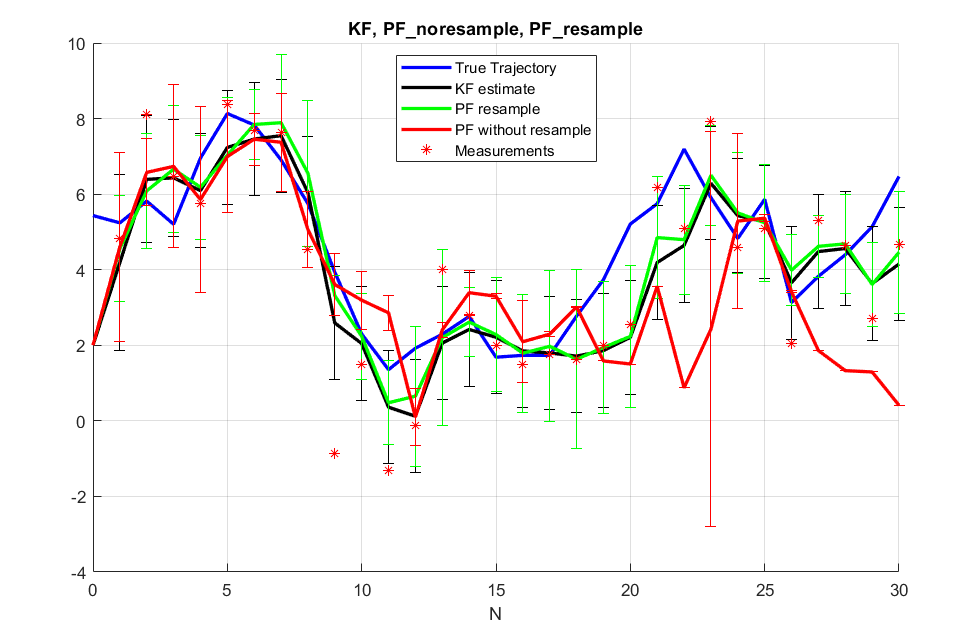
\includegraphics[width=0.7\textwidth]{images/pairfigure.png}
 \caption{The filter figure for these three steps}
 \label{S}
\end{figure}
  

However, the PF without resampling, on the other hand, does not update its particles based on their weights. Instead, it only performs the prediction and updates steps without resampling. This means that the particles are not adjusted to better represent the true posterior, potentially leading to a less accurate approximation. As the time step increases, the particles in the PF without resampling may deviate further from the true posterior, resulting in a larger discrepancy from the KF filter. Figure \ref{S} proves this. 

Overall, by selectively resampling particles based on their weights, the resampled PF can focus on regions of higher posterior probability and effectively track the true posterior distribution. 

\subsection{Task b}

\begin{figure}[H]
 \centering
 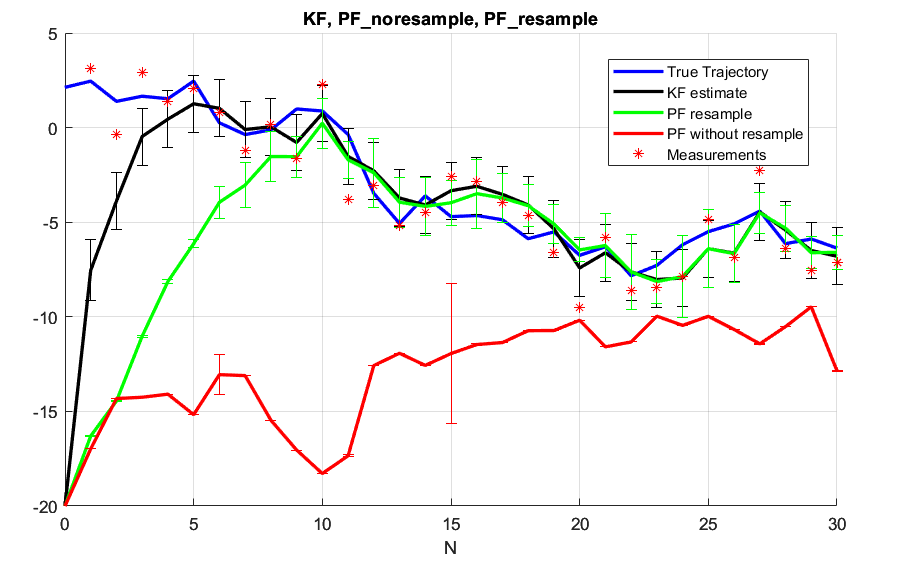
\includegraphics[width=0.7\textwidth]{images/wrongprior.png}
 \caption{Filters with wrong prior}
 \label{wrong}
\end{figure}

From figure \ref{wrong}, KF responds fastly and is the first one with these three filters that back to the correct position.

PF with resample is a little bit slower than the KF filter but it performs still well, and can finally converge to the real states curve.

Unfortunately, the PF without resample performs badly, even until the final step it can not back to an acceptable position.

The observation proves the analysis above in part 2, that compared with the other two,  the PF without resampling lacks an adaptive mechanism, leading to a less accurate approximation.

\subsection{c}

In this part, need to change the plot function or cannot draw particle filter with more than 50 particles.

\begin{figure}[H]
    \centering
    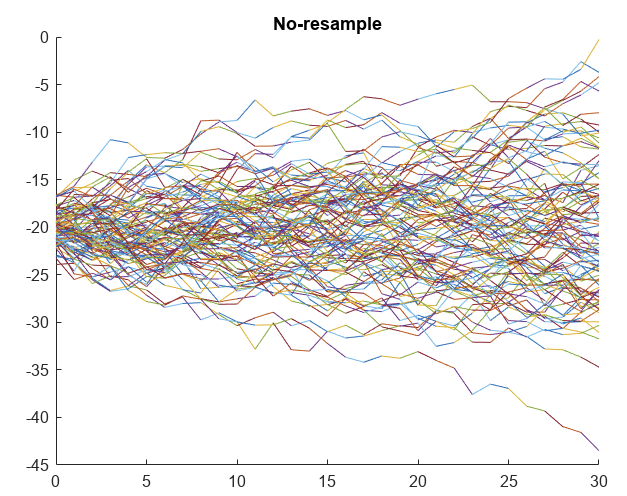
\includegraphics[width=0.7\textwidth]{images/withoutresample.png}
    \caption{without resample}
    \label{without}
   \end{figure}

When illustrating the particle trajectories for a PF without resampling, I observe that as the iterations progress, the particles continue to diverge and spread out without any convergence trend. This lack of convergence can be attributed to the absence of resampling. Without resampling, the particles are not being weighted according to their likelihoods, leading to an unbalanced distribution that fails to capture the true underlying state accurately. 

Consequently, the estimation performance of the filter is likely to deteriorate over time as the particles become increasingly scattered.


\subsection{d}



\begin{figure}[H]
    \centering
    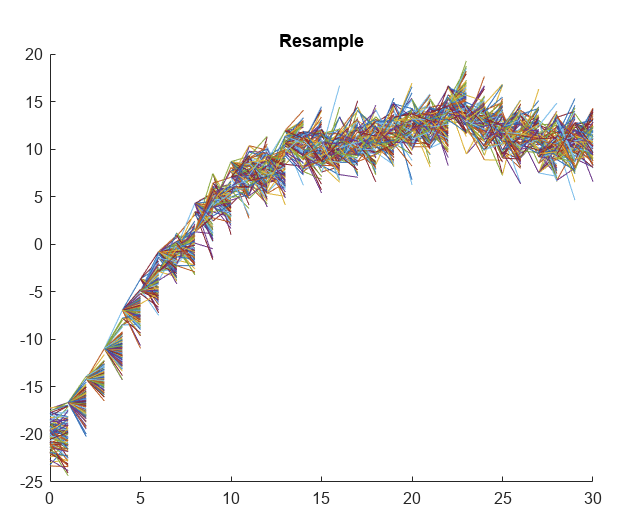
\includegraphics[width=0.7\textwidth]{images/resample.png}
    \caption{With resample}
    \label{resample}
   \end{figure}

   When illustrating the particle trajectories for a PF with resampling, initially, the particles are spread out, similar to the no-resampling case. However, as the iterations progress, the particles undergo resampling, which allows the more probable particles to be replicated and the less probable ones to be cut. This resampling process promotes the convergence of the particles toward the true underlying state. Consequently, I observe that the particle trajectories in the resampling case tend to cross and converge, indicating a better estimation performance compared to the no-resampling case. 